% ------------------------------------------------------------------------
%
% -------------------      Plantilla_UIS.tex       -----------------------
%
% ------------------------------------------------------------------------
% ------------------------------------------------------------------------
% ------------------------------------------------------------------------
% Versión de plantilla para realización de informes de trabajo de grado
% construida para uso de la Universidad Industrial de Santander.
%
% Reservados todos los derechos
%
% Bucaramanga, Colombia
%
% Septiembre 17 de 2018
%
% ------------------------------------------------------------------------
% ------------------------------------------------------------------------
% ------------------------------------------------------------------------
%
% ------------------------------------------------------------------------
\documentclass[letter,oneside,12pt,spanish, utf8]{report}          % Encabezados
% \usepackage[ansinew]{inputenc}
% \usepackage[spanish,es-nodecimaldot]{babel}

\usepackage[utf8]{inputenc}
% \usepackage[spanish]{babel}
\usepackage[spanish,es-nodecimaldot]{babel}

%\usepackage[latin]{babel}
% ------------------------------------------------------------------------
\usepackage{icontec_style}                   % Libreria UIS ICONTEC
% ------------------------------------------------------------------------
% Ingrese en este punto las librerías específicas de usuario
% ------------------------------------------------------------------------
\usepackage{amsmath}
\usepackage{amsthm}
\usepackage{amssymb}
\usepackage{subfigure}
\usepackage{hyperref}
\usepackage{float}
\usepackage{graphicx}
\usepackage{algorithm,algpseudocode}
\usepackage{xcolor}
\usepackage{multicol}
\usepackage{multirow}
%\usepackage[block=ragged]{biblatex}
%\usepackage{ulem}
\setcounter{tocdepth}{4} % show also subsections in toc
\setcounter{secnumdepth}{4} % show also subsections number in toc
% ------------------------------------------------------------------------
% Archivo de bibliografía
% ------------------------------------------------------------------------
\addbibresource{references.bib}
% ------------------------------------------------------------------------
\def\autor{NOMBRE DEL AUTOR}
\def\titulo{TITULO DEL TRABAJO}
\def\director{NOMBRE DIRECTOR}
\def\codirector{NOMBRE CODIRECTOR}
\def\universidad{Universidad Industrial de Santander}
\def\escuela{Escuela de NOMBRE DE LA ESCUELA}
\def\facultad{Facultad de NOMBRE DE LA FACULTAD}
\def\grupo{Grupo de Investigación en Diseño de Algoritmos y Procesamiento de Datos Multidimensionales (HDSP)}
\def\fecha{<NUMERO AÑO>}
\def\codigo{CODIGO ESTUDIANTE}

\DeclareMathOperator*{\minimize}{minimizar} % Declaración operador minimize

\DeclareMathOperator*{\maximize}{maximizar} % Declaración operador maximize
\DeclareMathOperator*{\subjectto}{sujeto \ a} % Declaración operador subjectto
\DeclareMathOperator*{\argmax}{arg \ max} % Declaración operador arg max

\DeclareMathOperator*{\argmin}{arg \ min} % Declaración operador arg min

%\DeclareMathOperator*{\min}{min} % Declaración operador min

\newtheorem{definition}{Definición}% Declaración segmento definición matemática

%\DefineBibliographyStrings{spanish}{andothers={et~al\adddot}}
% Traducción de palabras reservadas del algoritmo a español
\newenvironment{algoritmo}[1][]
  {\begin{algorithm}[#1]
     \selectlanguage{spanish}%
     \floatname{algorithm}{Algoritmo}%
     \renewcommand{\algorithmicif}{\textbf{si}}%
     \renewcommand{\algorithmicthen}{\textbf{entonces}}%
     \renewcommand{\algorithmicend}{\textbf{fin}}%
     \renewcommand{\algorithmicfor}{\textbf{para}}%
     \renewcommand{\algorithmicdo}{\textbf{hacer}}%
     % Set other language requirements
  }
  {\end{algorithm}}

\begin{document}       

% Inicio de documento
% ------------------------------------------------------------------------
% Definición silábica de palabras
% ------------------------------------------------------------------------
\hyphenation{pro-por-cio-nal di-se-ño}
\hypersetup {pdfborder = {0 0 0}}
% ------------------------------------------------------------------------
% Elementos previos al contenido del trabajo
% ------------------------------------------------------------------------
% ------------------------------------------------------------------------
%                                 Portada
% ------------------------------------------------------------------------

\thispagestyle{empty}

\begin{center}

\MakeUppercase{\titulo} \vspace{7cm}

\MakeUppercase{\autor}\\
\vspace{7cm}

\MakeUppercase{\universidad}\\
\MakeUppercase{\facultad}\\
\MakeUppercase{\escuela}\\
BUCARAMANGA\\
\fecha\\

\end{center}

% ------------------------------------------------------------------------
%                              Contraportada
% ------------------------------------------------------------------------

\newpage
\thispagestyle{empty}

\begin{center}

\MakeUppercase{\titulo} \vspace{2.3cm}

\MakeUppercase{\autor}\\
\vspace{2.3cm}

Trabajo de Grado para optar al título de\\
NOMBRE DEL PROGRAMA\\\vspace{1.5cm}

Director:\\
\director\\
\textit{Magíster/Ph.D. en NOMBRE DEL PROGRAMA}\vspace{0.5cm}

Codirector:\\
\codirector\\
\textit{Magíster/Ph.D. en NOMBRE DEL PROGRAMA} \vspace{1.5cm}

\MakeUppercase{\universidad}\\
\MakeUppercase{\facultad}\\
\MakeUppercase{\escuela}\\
BUCARAMANGA\\
\fecha\\

\end{center}

% ------------------------------------------------------------------------
   % Portada, contraportada, formato de nota y autorización
% ------------------------------------------------------------------------
% ------------------------------------------------------------------------
% ------------------------------------------------------------------------
% ------------------------------------------------------------------------
%                               Dedicatoria
% ------------------------------------------------------------------------
% ------------------------------------------------------------------------
% ------------------------------------------------------------------------
\chapter*{DEDICATORIA}

 \begin{flushright}.
 
\textit{
Cuántas veces, amor, te amé sin verte y tal vez sin recuerdo,\\ 
sin reconocer tu mirada, sin mirarte, centaura,\\
en regiones contrarias, en un mediodía quemante:\\
eras sólo el aroma de los cereales que amo.\\
Tal vez te vi, te supuse al pasar levantando una copa\\
en Angola, a la luz de la luna de Junio,\\
o eras tú la cintura de aquella guitarra\\
que toqué en las tinieblas y sonó como el mar desmedido.\\
Te amé sin que yo lo supiera, y busqué tu memoria.\\
En las casas vacías entré con linterna a robar tu retrato.\\
Pero yo ya sabía cómo era. De pronto\\
mientras ibas conmigo te toqué y se detuvo mi vida:\\
frente a mis ojos estabas, reinándome, y reinas.\\
Como hoguera en los bosques el fuego es tu reino.\\
- Pablo Neruda, Soneto 22}
\end{flushright}


% ------------------------------------------------------------------------                                      % Dedicatoria
% ------------------------------------------------------------------------
% ------------------------------------------------------------------------
% ------------------------------------------------------------------------
% ------------------------------------------------------------------------
%                             AGRADECIMIENTOS
% ------------------------------------------------------------------------
% ------------------------------------------------------------------------
% ------------------------------------------------------------------------
\chapter*{AGRADECIMIENTOS}


Lorem ipsum dolor sit amet, consectetur adipiscing elit. Donec pharetra scelerisque pellentesque. Morbi dapibus sem a nibh aliquet porta. Quisque sed metus nunc. Nunc faucibus tellus sodales tortor vulputate gravida. Praesent eget nisi sem. Pellentesque non congue quam, vitae lobortis sem. Maecenas condimentum ornare elementum. Suspendisse non scelerisque ex. Mauris ultricies, enim et sagittis tristique, sem sem varius dolor, vel eleifend arcu velit non nibh. Vivamus malesuada pellentesque velit sit amet convallis.

Nam eget cursus mi, eget fringilla urna. Aenean eleifend sodales sem, eu facilisis eros finibus eu. Praesent eget ipsum ac eros pretium tincidunt. Integer iaculis egestas metus a interdum. Sed hendrerit enim diam, eu maximus diam condimentum quis. Suspendisse at accumsan magna. Donec sodales ultrices interdum. Nullam euismod dignissim tempus. Suspendisse viverra tempor est in egestas. Quisque scelerisque eleifend hendrerit. Sed mattis mollis purus, eget dapibus velit tempor a. Etiam at condimentum augue. Integer interdum erat mollis neque suscipit ultricies.


% ------------------------------------------------------------------------
\newpage                              % Agradecimientos
% ------------------------------------------------------------------------
\tableofcontents                                      % Tabla de contenido
% ------------------------------------------------------------------------
\listoffigures                         % Lista de figuras, tablas y anexos
\listoftables
%\listofanexo
% ------------------------------------------------------------------------
%\input{Secs/Glosario}                               % Glosario de términos
% ------------------------------------------------------------------------
% Contenido del Informe
% ------------------------------------------------------------------------
% ------------------------------------------------------------------------
% ------------------------------------------------------------------------
% ------------------------------------------------------------------------
%                                Resumen
% ------------------------------------------------------------------------
% ------------------------------------------------------------------------
% ------------------------------------------------------------------------
\chapter*{RESUMEN}

\footnotesize{
\begin{description}
  \item[TÍTULO:] \MakeUppercase{\titulo}
  \astfootnote{Trabajo de grado}
  \item[AUTOR:]\MakeUppercase{\autor} \asttfootnote{\facultad. \escuela. Director: \director. Codirector: \codirector.}
  \item[PALABRAS CLAVE:] Palabra Clave 1, Palabra Clave 2, Palabra Clave 3.
  \item[DESCRIPCIÓN:]\hfill \\ 
Lorem ipsum dolor sit amet, consectetur adipiscing elit. Donec pharetra scelerisque pellentesque. Morbi dapibus sem a nibh aliquet porta. Quisque sed metus nunc. Nunc faucibus tellus sodales tortor vulputate gravida. Praesent eget nisi sem. Pellentesque non congue quam, vitae lobortis sem. Maecenas condimentum ornare elementum. Suspendisse non scelerisque ex. Mauris ultricies, enim et sagittis tristique, sem sem varius dolor, vel eleifend arcu velit non nibh. Vivamus malesuada pellentesque velit sit amet convallis.Nam eget cursus mi, eget fringilla urna. Aenean eleifend sodales sem, eu facilisis eros finibus eu. Praesent eget ipsum ac eros pretium tincidunt. Integer iaculis egestas metus a interdum. Sed hendrerit enim diam, eu maximus diam condimentum quis. Suspendisse at accumsan magna. Donec sodales ultrices interdum. Nullam euismod dignissim tempus. Suspendisse viverra tempor est in egestas. Quisque scelerisque eleifend hendrerit. Sed mattis mollis purus, eget dapibus velit tempor a. Etiam at condimentum augue. Integer interdum erat mollis neque suscipit ultricies. Fusce tincidunt risus augue, eget egestas metus commodo sed. Suspendisse id nisl efficitur, pellentesque lorem eu, pellentesque lacus. Vivamus ullamcorper nibh eu ultricies pulvinar. Donec accumsan magna mauris, in lobortis lacus ornare ac. Curabitur semper sem sed ornare fringilla. Ut bibendum velit non ante pharetra dignissim. Praesent eget vehicula odio. Donec lobortis sed libero id tempus. Nunc vehicula a ligula eget mattis. Aenean porttitor odio et justo fermentum malesuada. Proin auctor lorem eget velit facilisis consequat. Proin et ex lorem. Cras hendrerit leo vel eros ornare, in fringilla augue sollicitudin. Nunc efficitur purus vel nisi pellentesque volutpat. Aenean ultricies, ligula sit amet eleifend convallis, lacus est scelerisque nisl, eget consectetur leo lacus nec enim.
\end{description}}\normalsize
% ------------------------------------------------------------------------                                                % Resumen

\chapter*{ABSTRACT}

\footnotesize{
\begin{description}
  \item[TITLE:] TITLE IN ENGLISH APPROACH\astfootnote{Bachelor Thesis}
  \item[AUTHOR:] \MakeUppercase{\autor} \asttfootnote{\facultad. \escuela. Advisor: \director. Co-advisor: \codirector}
  \item[KEYWORDS:] Keyword 1, Keyword 2, Keyword 3.
  \item[DESCRIPTION:]\hfill \\ Lorem ipsum dolor sit amet, consectetur adipiscing elit. Donec pharetra scelerisque pellentesque. Morbi dapibus sem a nibh aliquet porta. Quisque sed metus nunc. Nunc faucibus tellus sodales tortor vulputate gravida. Praesent eget nisi sem. Pellentesque non congue quam, vitae lobortis sem. Maecenas condimentum ornare elementum. Suspendisse non scelerisque ex. Mauris ultricies, enim et sagittis tristique, sem sem varius dolor, vel eleifend arcu velit non nibh. Vivamus malesuada pellentesque velit sit amet convallis.Nam eget cursus mi, eget fringilla urna. Aenean eleifend sodales sem, eu facilisis eros finibus eu. Praesent eget ipsum ac eros pretium tincidunt. Integer iaculis egestas metus a interdum. Sed hendrerit enim diam, eu maximus diam condimentum quis. Suspendisse at accumsan magna. Donec sodales ultrices interdum. Nullam euismod dignissim tempus. Suspendisse viverra tempor est in egestas. Quisque scelerisque eleifend hendrerit. Sed mattis mollis purus, eget dapibus velit tempor a. Etiam at condimentum augue. Integer interdum erat mollis neque suscipit ultricies. Fusce tincidunt risus augue, eget egestas metus commodo sed. Suspendisse id nisl efficitur, pellentesque lorem eu, pellentesque lacus. Vivamus ullamcorper nibh eu ultricies pulvinar. Donec accumsan magna mauris, in lobortis lacus ornare ac. Curabitur semper sem sed ornare fringilla. Ut bibendum velit non ante pharetra dignissim. Praesent eget vehicula odio. Donec lobortis sed libero id tempus. Nunc vehicula a ligula eget mattis. Aenean porttitor odio et justo fermentum malesuada. Proin auctor lorem eget velit facilisis consequat. Proin et ex lorem. Cras hendrerit leo vel eros ornare, in fringilla augue sollicitudin. Nunc efficitur purus vel nisi pellentesque volutpat. Aenean ultricies, ligula sit amet eleifend convallis, lacus est scelerisque nisl, eget consectetur leo lacus nec enim.
\end{description}}\normalsize
% ------------------------------------------------------------------------                                               % Abstract
% ------------------------------------------------------------------------
% Capítulos
% ------------------------------------------------------------------------
% Introducción


\nnchapter{INTRODUCCIÓN}


Lorem ipsum dolor sit amet, consectetur adipiscing elit. Donec pharetra scelerisque pellentesque. Morbi dapibus sem a nibh aliquet porta. Quisque sed metus nunc. Nunc faucibus tellus sodales tortor vulputate gravida. Praesent eget nisi sem. Pellentesque non congue quam, vitae lobortis sem. Maecenas condimentum ornare elementum. Suspendisse non scelerisque ex. Mauris ultricies, enim et sagittis tristique, sem sem varius dolor, vel eleifend arcu velit non nibh. Vivamus malesuada pellentesque velit sit amet convallis~\myfootcite{xiao2017fashion}.

Nam eget cursus mi, eget fringilla urna. Aenean eleifend sodales sem, eu facilisis eros finibus eu. Praesent eget ipsum ac eros pretium tincidunt. Integer iaculis egestas metus a interdum. Sed hendrerit enim diam, eu maximus diam condimentum quis. Suspendisse at accumsan magna. Donec sodales ultrices interdum. Nullam euismod dignissim tempus. Suspendisse viverra tempor est in egestas. Quisque scelerisque eleifend hendrerit. Sed mattis mollis purus, eget dapibus velit tempor a. Etiam at condimentum augue. Integer interdum erat mollis neque suscipit ultricies~\myfootcite{deng2012mnist}.

Fusce tincidunt risus augue, eget egestas metus commodo sed. Suspendisse id nisl efficitur, pellentesque lorem eu, pellentesque lacus. Vivamus ullamcorper nibh eu ultricies pulvinar. Donec accumsan magna mauris, in lobortis lacus ornare ac. Curabitur semper sem sed ornare fringilla. Ut bibendum velit non ante pharetra dignissim. Praesent eget vehicula odio. Donec lobortis sed libero id tempus. Nunc vehicula a ligula eget mattis. Aenean porttitor odio et justo fermentum malesuada. Proin auctor lorem eget velit facilisis consequat. Proin et ex lorem. Cras hendrerit leo vel eros ornare, in fringilla augue sollicitudin. Nunc efficitur purus vel nisi pellentesque volutpat. Aenean ultricies, ligula sit amet eleifend convallis, lacus est scelerisque nisl, eget consectetur leo lacus nec enim~\myfootcite{inceptionv3}.

Suspendisse turpis massa, faucibus a purus a, condimentum venenatis turpis. Maecenas nec lorem suscipit, accumsan neque in, iaculis quam. Sed sit amet lorem odio. Duis euismod metus nec tellus ultricies, in vehicula mi consequat. Nullam nisl mauris, lacinia ut ornare quis, consequat et nisi. Proin quis turpis sem. Cras nisi lorem, rutrum id elit eget, consectetur semper quam.

Pellentesque vitae accumsan diam. Lorem ipsum dolor sit amet, consectetur adipiscing elit. Donec gravida viverra eros, id sodales nisi egestas id. Etiam faucibus in enim at efficitur. In ac tincidunt nulla. Sed eget massa purus. Sed eu augue vitae diam congue rutrum. Integer neque enim, facilisis eget neque venenatis, efficitur tincidunt nibh. Fusce ullamcorper magna ante, vitae faucibus felis facilisis at. Phasellus at velit lacus. Donec vitae condimentum tellus. Donec sagittis consectetur mollis. Ut ullamcorper elementum facilisis.


%\pagebreak % Introducción
% ------------------------------------------------------------------------
% ------------------------------------------------------------------------
% ------------------------------------------------------------------------
%                              Objetivos
% ------------------------------------------------------------------------
% ------------------------------------------------------------------------
% ------------------------------------------------------------------------

\chapter{OBJETIVOS}

\subsection*{Objetivo general}

\begin{itemize}
   \item Lorem ipsum dolor sit amet, consectetur adipiscing elit. Donec pharetra scelerisque pellentesque. Morbi dapibus sem a nibh aliquet porta. Quisque sed metus nunc. 
\end{itemize}

\subsection*{Objetivos específicos}


\begin{enumerate}

    \item Lorem ipsum dolor sit amet, consectetur adipiscing elit. Donec pharetra scelerisque pellentesque. Morbi dapibus sem a nibh aliquet porta. Quisque sed metus nunc. 

    \item Lorem ipsum dolor sit amet, consectetur adipiscing elit. Donec pharetra scelerisque pellentesque. Morbi dapibus sem a nibh aliquet porta. Quisque sed metus nunc. 
    
    \item Lorem ipsum dolor sit amet, consectetur adipiscing elit. Donec pharetra scelerisque pellentesque. Morbi dapibus sem a nibh aliquet porta. Quisque sed metus nunc. 
    
    \item Lorem ipsum dolor sit amet, consectetur adipiscing elit. Donec pharetra scelerisque pellentesque. Morbi dapibus sem a nibh aliquet porta. Quisque sed metus nunc. 

\end{enumerate}
\pagebreak


% ------------------------------------------------------------------------
% ------------------------------------------------------------------------  % Objetivos
\chapter{EJEMPLO SECCIÓN}

Lorem ipsum dolor sit amet, consectetur adipiscing elit. Donec pharetra scelerisque pellentesque. Morbi dapibus sem a nibh aliquet porta. Quisque sed metus nunc. Nunc faucibus tellus sodales tortor vulputate gravida. Praesent eget nisi sem~\myfootcite{pinilla2018coded}. Pellentesque non congue quam, vitae lobortis sem. Maecenas condimentum ornare elementum. Suspendisse non scelerisque ex. Mauris ultricies, enim et sagittis tristique, sem sem varius dolor, vel eleifend arcu velit non nibh. Vivamus malesuada pellentesque velit sit amet convallis~\myfootcite{fienup1987phase}.


    
\section{EJEMPLO SUBSECCIÓN}

Lorem ipsum dolor sit amet, consectetur adipiscing elit. Donec pharetra scelerisque pellentesque. Morbi dapibus sem a nibh aliquet porta. Quisque sed metus nunc. Nunc faucibus tellus sodales tortor vulputate gravida. Praesent eget nisi sem. Pellentesque non congue quam, vitae lobortis sem. Maecenas condimentum ornare elementum. Suspendisse non scelerisque ex. Mauris ultricies, enim et sagittis tristique, sem sem varius dolor, vel eleifend arcu velit non nibh. Vivamus malesuada pellentesque velit sit amet convallis.

\begin{figure}[!h]
    \centering
    \caption{\hspace{2mm}Ejemplo Figure: Sistema óptico de difracción convencional.}
    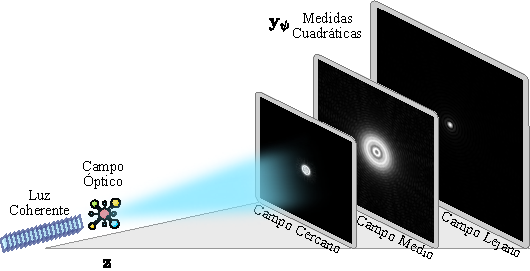
\includegraphics[width=0.9\linewidth]{images/marco_teórico/diffraction_no_coded.pdf}
    \label{fig:difraction_systems}
\end{figure}

EJEMPLO ECUACIÓN 1

\begin{equation}
    \mathbf{y}_{\psi}= \vert \mathbf{A}_\psi \mathbf{z} \vert^2,
    \label{eq:diffraction_base}
\end{equation}


EJEMPLO ECUACIÓN 2

\begin{equation}
    \mathbf{A}_\psi = \left\{\begin{matrix}
 \mathbf{F}\mathbf{T}\mathbf{F}^\mathcal{H}    & \text{si } \psi=1\rightarrow \text{Campo cercano},\\ 
 \mathbf{F}^\mathcal{H}\mathbf{Q} &\text{si } \psi=2\rightarrow\text{ Campo medio}, \\ 
 \mathbf{F}  &\text{si } \psi=3\rightarrow\text{Campo lejano},
\end{matrix}\right. \label{eq:matrix_a_no_coded}
\end{equation}

Nam eget cursus mi, eget fringilla urna. Aenean eleifend sodales sem, eu facilisis eros finibus eu. Praesent eget ipsum ac eros pretium tincidunt. Integer iaculis egestas metus a interdum. Sed hendrerit enim diam, eu maximus diam condimentum quis. Suspendisse at accumsan magna. Donec sodales ultrices interdum. Nullam euismod dignissim tempus. Suspendisse viverra tempor est in egestas. Quisque scelerisque eleifend hendrerit. Sed mattis mollis purus, eget dapibus velit tempor a. Etiam at condimentum augue. Integer interdum erat mollis neque suscipit ultricies.


 % Marco de referencia
% ------------------------------------------------------------------------
% ------------------------------------------------------------------------
% ------------------------------------------------------------------------
%                                Capítulo 3
% ------------------------------------------------------------------------
% ------------------------------------------------------------------------
% ------------------------------------------------------------------------

\chapter{METODOLOGÍA PROPUESTA}


Lorem ipsum dolor sit amet, consectetur adipiscing elit. Donec pharetra scelerisque pellentesque. Morbi dapibus sem a nibh aliquet porta. Quisque sed metus nunc. Nunc faucibus tellus sodales tortor vulputate gravida. Praesent eget nisi sem. Pellentesque non congue quam, vitae lobortis sem. Maecenas condimentum ornare elementum. Suspendisse non scelerisque ex. Mauris ultricies, enim et sagittis tristique, sem sem varius dolor, vel eleifend arcu velit non nibh. Vivamus malesuada pellentesque velit sit amet convallis.

\section{SUBSECCION}
Lorem ipsum dolor sit amet, consectetur adipiscing elit. Donec pharetra scelerisque pellentesque. Morbi dapibus sem a nibh aliquet porta. Quisque sed metus nunc. Nunc faucibus tellus sodales tortor vulputate gravida. Praesent eget nisi sem. Pellentesque non congue quam, vitae lobortis sem. Maecenas condimentum ornare elementum. Suspendisse non scelerisque ex. Mauris ultricies, enim et sagittis tristique, sem sem varius dolor, vel eleifend arcu velit non nibh. Vivamus malesuada pellentesque velit sit amet convallis.

Nam eget cursus mi, eget fringilla urna. Aenean eleifend sodales sem, eu facilisis eros finibus eu. Praesent eget ipsum ac eros pretium tincidunt. Integer iaculis egestas metus a interdum. Sed hendrerit enim diam, eu maximus diam condimentum quis. Suspendisse at accumsan magna. Donec sodales ultrices interdum. Nullam euismod dignissim tempus. Suspendisse viverra tempor est in egestas. Quisque scelerisque eleifend hendrerit. Sed mattis mollis purus, eget dapibus velit tempor a. Etiam at condimentum augue. Integer interdum erat mollis neque suscipit ultricies.

Fusce tincidunt risus augue, eget egestas metus commodo sed. Suspendisse id nisl efficitur, pellentesque lorem eu, pellentesque lacus. Vivamus ullamcorper nibh eu ultricies pulvinar. Donec accumsan magna mauris, in lobortis lacus ornare ac. Curabitur semper sem sed ornare fringilla. Ut bibendum velit non ante pharetra dignissim. Praesent eget vehicula odio. Donec lobortis sed libero id tempus. Nunc vehicula a ligula eget mattis. Aenean porttitor odio et justo fermentum malesuada. Proin auctor lorem eget velit facilisis consequat. Proin et ex lorem. Cras hendrerit leo vel eros ornare, in fringilla augue sollicitudin. Nunc efficitur purus vel nisi pellentesque volutpat. Aenean ultricies, ligula sit amet eleifend convallis, lacus est scelerisque nisl, eget consectetur leo lacus nec enim.

\section{SUBSECCION}
Lorem ipsum dolor sit amet, consectetur adipiscing elit. Donec pharetra scelerisque pellentesque. Morbi dapibus sem a nibh aliquet porta. Quisque sed metus nunc. Nunc faucibus tellus sodales tortor vulputate gravida. Praesent eget nisi sem. Pellentesque non congue quam, vitae lobortis sem. Maecenas condimentum ornare elementum. Suspendisse non scelerisque ex. Mauris ultricies, enim et sagittis tristique, sem sem varius dolor, vel eleifend arcu velit non nibh. Vivamus malesuada pellentesque velit sit amet convallis.

Nam eget cursus mi, eget fringilla urna. Aenean eleifend sodales sem, eu facilisis eros finibus eu. Praesent eget ipsum ac eros pretium tincidunt. Integer iaculis egestas metus a interdum. Sed hendrerit enim diam, eu maximus diam condimentum quis. Suspendisse at accumsan magna. Donec sodales ultrices interdum. Nullam euismod dignissim tempus. Suspendisse viverra tempor est in egestas. Quisque scelerisque eleifend hendrerit. Sed mattis mollis purus, eget dapibus velit tempor a. Etiam at condimentum augue. Integer interdum erat mollis neque suscipit ultricies.

Fusce tincidunt risus augue, eget egestas metus commodo sed. Suspendisse id nisl efficitur, pellentesque lorem eu, pellentesque lacus. Vivamus ullamcorper nibh eu ultricies pulvinar. Donec accumsan magna mauris, in lobortis lacus ornare ac. Curabitur semper sem sed ornare fringilla. Ut bibendum velit non ante pharetra dignissim. Praesent eget vehicula odio. Donec lobortis sed libero id tempus. Nunc vehicula a ligula eget mattis. Aenean porttitor odio et justo fermentum malesuada. Proin auctor lorem eget velit facilisis consequat. Proin et ex lorem. Cras hendrerit leo vel eros ornare, in fringilla augue sollicitudin. Nunc efficitur purus vel nisi pellentesque volutpat. Aenean ultricies, ligula sit amet eleifend convallis, lacus est scelerisque nisl, eget consectetur leo lacus nec enim.

\section{SUBSECCION}
Lorem ipsum dolor sit amet, consectetur adipiscing elit. Donec pharetra scelerisque pellentesque. Morbi dapibus sem a nibh aliquet porta. Quisque sed metus nunc. Nunc faucibus tellus sodales tortor vulputate gravida. Praesent eget nisi sem. Pellentesque non congue quam, vitae lobortis sem. Maecenas condimentum ornare elementum. Suspendisse non scelerisque ex. Mauris ultricies, enim et sagittis tristique, sem sem varius dolor, vel eleifend arcu velit non nibh. Vivamus malesuada pellentesque velit sit amet convallis.

Nam eget cursus mi, eget fringilla urna. Aenean eleifend sodales sem, eu facilisis eros finibus eu. Praesent eget ipsum ac eros pretium tincidunt. Integer iaculis egestas metus a interdum. Sed hendrerit enim diam, eu maximus diam condimentum quis. Suspendisse at accumsan magna. Donec sodales ultrices interdum. Nullam euismod dignissim tempus. Suspendisse viverra tempor est in egestas. Quisque scelerisque eleifend hendrerit. Sed mattis mollis purus, eget dapibus velit tempor a. Etiam at condimentum augue. Integer interdum erat mollis neque suscipit ultricies.

Fusce tincidunt risus augue, eget egestas metus commodo sed. Suspendisse id nisl efficitur, pellentesque lorem eu, pellentesque lacus. Vivamus ullamcorper nibh eu ultricies pulvinar. Donec accumsan magna mauris, in lobortis lacus ornare ac. Curabitur semper sem sed ornare fringilla. Ut bibendum velit non ante pharetra dignissim. Praesent eget vehicula odio. Donec lobortis sed libero id tempus. Nunc vehicula a ligula eget mattis. Aenean porttitor odio et justo fermentum malesuada. Proin auctor lorem eget velit facilisis consequat. Proin et ex lorem. Cras hendrerit leo vel eros ornare, in fringilla augue sollicitudin. Nunc efficitur purus vel nisi pellentesque volutpat. Aenean ultricies, ligula sit amet eleifend convallis, lacus est scelerisque nisl, eget consectetur leo lacus nec enim. % Modelo matemático del DRON
% ------------------------------------------------------------------------
% ------------------------------------------------------------------------
% ------------------------------------------------------------------------
%                                Capítulo 4
% ------------------------------------------------------------------------
% ------------------------------------------------------------------------
% ------------------------------------------------------------------------

\chapter{SIMULACIONES Y RESULTADOS}

Lorem ipsum dolor sit amet, consectetur adipiscing elit. Donec pharetra scelerisque pellentesque. Morbi dapibus sem a nibh aliquet porta. Quisque sed metus nunc. Nunc faucibus tellus sodales tortor vulputate gravida. Praesent eget nisi sem. Pellentesque non congue quam, vitae lobortis sem. Maecenas condimentum ornare elementum. Suspendisse non scelerisque ex. Mauris ultricies, enim et sagittis tristique, sem sem varius dolor, vel eleifend arcu velit non nibh. Vivamus malesuada pellentesque velit sit amet convallis.


\section{CONJUNTO DE DATOS}
Lorem ipsum dolor sit amet, consectetur adipiscing elit. Donec pharetra scelerisque pellentesque. Morbi dapibus sem a nibh aliquet porta. Quisque sed metus nunc. Nunc faucibus tellus sodales tortor vulputate gravida. Praesent eget nisi sem. Pellentesque non congue quam, vitae lobortis sem. Maecenas condimentum ornare elementum. Suspendisse non scelerisque ex. Mauris ultricies, enim et sagittis tristique, sem sem varius dolor, vel eleifend arcu velit non nibh. Vivamus malesuada pellentesque velit sit amet convallis.

Nam eget cursus mi, eget fringilla urna. Aenean eleifend sodales sem, eu facilisis eros finibus eu. Praesent eget ipsum ac eros pretium tincidunt. Integer iaculis egestas metus a interdum. Sed hendrerit enim diam, eu maximus diam condimentum quis. Suspendisse at accumsan magna. Donec sodales ultrices interdum. Nullam euismod dignissim tempus. Suspendisse viverra tempor est in egestas. Quisque scelerisque eleifend hendrerit. Sed mattis mollis purus, eget dapibus velit tempor a. Etiam at condimentum augue. Integer interdum erat mollis neque suscipit ultricies.

Fusce tincidunt risus augue, eget egestas metus commodo sed. Suspendisse id nisl efficitur, pellentesque lorem eu, pellentesque lacus. Vivamus ullamcorper nibh eu ultricies pulvinar. Donec accumsan magna mauris, in lobortis lacus ornare ac. Curabitur semper sem sed ornare fringilla. Ut bibendum velit non ante pharetra dignissim. Praesent eget vehicula odio. Donec lobortis sed libero id tempus. Nunc vehicula a ligula eget mattis. Aenean porttitor odio et justo fermentum malesuada. Proin auctor lorem eget velit facilisis consequat. Proin et ex lorem. Cras hendrerit leo vel eros ornare, in fringilla augue sollicitudin. Nunc efficitur purus vel nisi pellentesque volutpat. Aenean ultricies, ligula sit amet eleifend convallis, lacus est scelerisque nisl, eget consectetur leo lacus nec enim.

\section{MÉTRICAS}

Lorem ipsum dolor sit amet, consectetur adipiscing elit. Donec pharetra scelerisque pellentesque. Morbi dapibus sem a nibh aliquet porta. Quisque sed metus nunc. Nunc faucibus tellus sodales tortor vulputate gravida. Praesent eget nisi sem. Pellentesque non congue quam, vitae lobortis sem. Maecenas condimentum ornare elementum. Suspendisse non scelerisque ex. Mauris ultricies, enim et sagittis tristique, sem sem varius dolor, vel eleifend arcu velit non nibh. Vivamus malesuada pellentesque velit sit amet convallis.

Nam eget cursus mi, eget fringilla urna. Aenean eleifend sodales sem, eu facilisis eros finibus eu. Praesent eget ipsum ac eros pretium tincidunt. Integer iaculis egestas metus a interdum. Sed hendrerit enim diam, eu maximus diam condimentum quis. Suspendisse at accumsan magna. Donec sodales ultrices interdum. Nullam euismod dignissim tempus. Suspendisse viverra tempor est in egestas. Quisque scelerisque eleifend hendrerit. Sed mattis mollis purus, eget dapibus velit tempor a. Etiam at condimentum augue. Integer interdum erat mollis neque suscipit ultricies.

Fusce tincidunt risus augue, eget egestas metus commodo sed. Suspendisse id nisl efficitur, pellentesque lorem eu, pellentesque lacus. Vivamus ullamcorper nibh eu ultricies pulvinar. Donec accumsan magna mauris, in lobortis lacus ornare ac. Curabitur semper sem sed ornare fringilla. Ut bibendum velit non ante pharetra dignissim. Praesent eget vehicula odio. Donec lobortis sed libero id tempus. Nunc vehicula a ligula eget mattis. Aenean porttitor odio et justo fermentum malesuada. Proin auctor lorem eget velit facilisis consequat. Proin et ex lorem. Cras hendrerit leo vel eros ornare, in fringilla augue sollicitudin. Nunc efficitur purus vel nisi pellentesque volutpat. Aenean ultricies, ligula sit amet eleifend convallis, lacus est scelerisque nisl, eget consectetur leo lacus nec enim.

\section{EXPERIMENTOS}
Lorem ipsum dolor sit amet, consectetur adipiscing elit. Donec pharetra scelerisque pellentesque. Morbi dapibus sem a nibh aliquet porta. Quisque sed metus nunc. Nunc faucibus tellus sodales tortor vulputate gravida. Praesent eget nisi sem. Pellentesque non congue quam, vitae lobortis sem. Maecenas condimentum ornare elementum. Suspendisse non scelerisque ex. Mauris ultricies, enim et sagittis tristique, sem sem varius dolor, vel eleifend arcu velit non nibh. Vivamus malesuada pellentesque velit sit amet convallis.

Nam eget cursus mi, eget fringilla urna. Aenean eleifend sodales sem, eu facilisis eros finibus eu. Praesent eget ipsum ac eros pretium tincidunt. Integer iaculis egestas metus a interdum. Sed hendrerit enim diam, eu maximus diam condimentum quis. Suspendisse at accumsan magna. Donec sodales ultrices interdum. Nullam euismod dignissim tempus. Suspendisse viverra tempor est in egestas. Quisque scelerisque eleifend hendrerit. Sed mattis mollis purus, eget dapibus velit tempor a. Etiam at condimentum augue. Integer interdum erat mollis neque suscipit ultricies.



\subsection{Configuración experimental.}

Lorem ipsum dolor sit amet, consectetur adipiscing elit. Donec pharetra scelerisque pellentesque. Morbi dapibus sem a nibh aliquet porta. Quisque sed metus nunc. Nunc faucibus tellus sodales tortor vulputate gravida. Praesent eget nisi sem. Pellentesque non congue quam, vitae lobortis sem. Maecenas condimentum ornare elementum. Suspendisse non scelerisque ex. Mauris ultricies, enim et sagittis tristique, sem sem varius dolor, vel eleifend arcu velit non nibh. Vivamus malesuada pellentesque velit sit amet convallis.

Nam eget cursus mi, eget fringilla urna. Aenean eleifend sodales sem, eu facilisis eros finibus eu. Praesent eget ipsum ac eros pretium tincidunt. Integer iaculis egestas metus a interdum. Sed hendrerit enim diam, eu maximus diam condimentum quis. Suspendisse at accumsan magna. Donec sodales ultrices interdum. Nullam euismod dignissim tempus. Suspendisse viverra tempor est in egestas. Quisque scelerisque eleifend hendrerit. Sed mattis mollis purus, eget dapibus velit tempor a. Etiam at condimentum augue. Integer interdum erat mollis neque suscipit ultricies.
 % Controladores PI y su conjunto estabilizante
% ------------------------------------------------------------------------
% ------------------------------------------------------------------------
% ------------------------------------------------------------------------
%                             Conclusiones
% ------------------------------------------------------------------------
% ------------------------------------------------------------------------
% ------------------------------------------------------------------------

\chapter{CONCLUSIONES}


Lorem ipsum dolor sit amet, consectetur adipiscing elit. Praesent luctus ornare justo eget lacinia. Cras laoreet dictum metus vitae commodo. Sed pellentesque ullamcorper orci in efficitur. Vivamus a velit quam. Nam euismod in odio vitae sodales. Cras in molestie tortor. Aliquam sed lectus dui. Duis quis nibh viverra, eleifend ex sed, mattis ipsum.

Praesent at semper tortor. Pellentesque commodo nisi nec nibh porta porta vitae quis dolor. Nulla mattis odio eget maximus rhoncus. Praesent dapibus mattis lorem vitae auctor. Vivamus eu tortor leo. Cras ut velit odio. Vestibulum in finibus mi. Vivamus eu magna lacus. Etiam gravida consectetur vulputate. Nulla semper justo sagittis venenatis semper.

Sed eu velit non enim tincidunt iaculis. Vestibulum eget vehicula quam. Maecenas non odio at ligula eleifend imperdiet. Donec arcu est, rutrum sit amet diam non, rhoncus eleifend mauris. Integer non interdum orci, non molestie metus. Mauris sed mi odio. Pellentesque vestibulum libero in dapibus volutpat. Fusce eget ullamcorper mi, sed commodo nulla. Nam bibendum enim vulputate purus hendrerit, nec sollicitudin nisl pellentesque. Mauris ut orci risus. In quis vestibulum turpis. Duis iaculis felis non lectus porttitor convallis. Suspendisse velit sem, tempus sit amet semper sed, fringilla sit amet urna. Nam ut accumsan nulla, ac vulputate massa. % Conclusiones
% ------------------------------------------------------------------------
% ------------------------------------------------------------------------
% ------------------------------------------------------------------------
%                            Trabajo futuro
% ------------------------------------------------------------------------
% ------------------------------------------------------------------------
% ------------------------------------------------------------------------

\chapter{TRABAJO FUTURO}
% ------------------------------------------------------------------------
% \noindent Actividades complementarias a los desarrollos presentados, incluyen el cálculo automático para conjuntos estabilizantes en plantas arbitrarias empleando el \emph{método de la signatura} desarrollado por Keel y Bhattacharyya en \myfootcite{keel2008}.\\

% Asimismo es importante explorar otras topologias de compensador y controladores PID, en sus versiones de tiempo continuo y discreto.
% ------------------------------------------------------------------------

El método propuesto puede llegar a ser validado experimentalmente mediante la implementación de un sistema óptico de adquisición de medidas cuadráticas codificadas. Adicionalmente, en este trabajo se realizó la inclusión de una capa que simula el proceso de adquisición de las medidas, por lo tanto, se abre la posibilidad de introducir una máscara de codificación $\mathbf{D}_\ell$ entrenable dentro del esquema de red neuronal, con el objetivo de determinar una codificación óptima que mejore el proceso de clasificación.
 % Trabajo futuro

% ------------------------------------------------------------------------
% Bibliografía
% ------------------------------------------------------------------------
\printbibliography[heading=bibintoc,title={BIBLIOGRAFÍA},omitnumbers=true]
% ------------------------------------------------------------------------
% Anexos
% ------------------------------------------------------------------------
% \input{Secs/anexoA} % Fundamentos de sólidos rígidos
% \input{Secs/anexoB} % Función ode45 de MATLAB
% \input{Secs/anexoC} % Interfaz de animación de la dinámica del sistema
% ------------------------------------------------------------------------
\end{document}                                          % Fin de documento
% ------------------------------------------------------------------------ 